\documentclass[12pt]{report}  

\pagestyle{empty}

\usepackage{graphics}
\usepackage{amsmath,amssymb,amsthm, multicol,array}
\usepackage[pdftex]{graphicx}
\usepackage{enumerate}
\usepackage{epsf}

\theoremstyle{definition}
\newtheorem{thm}{Theorem}
\newtheorem{lem}[thm]{Lemma}
\newtheorem{cor}[thm]{Corollary}
\newtheorem{rem}[thm]{Remark}
\newtheorem{remark}[thm]{Remark}
\newtheorem{conj}[thm]{Conjecture}
\newtheorem{definition}[thm]{Definition}

\newcommand{\naturals}{\mathbb{N}}
\newcommand{\integers}{\mathbb{Z}}
\newcommand{\complex}{\mathbb{C}}
\newcommand{\reals}{\mathbb{R}}
\newcommand{\mcal}[1]{\mathcal{#1}}
\newcommand{\rationals}{\mathbb{Q}}
\newcommand{\Aut}{\text{Aut}}
\newcommand{\Lp}[2]{\left\|{#1}\right\|_{L^{#2}}}
\newcommand{\tr}{\text{tr}}
\newcommand{\field}{\mathbb{F}}

\addtolength{\oddsidemargin}{-.75in}
\addtolength{\evensidemargin}{-.75in}
\addtolength{\textwidth}{1.5in}
\addtolength{\topmargin}{-1in}
\addtolength{\textheight}{2.25in}

\begin{document}
\begin{center}
{\bf \Large Math 13 - Week 4: More on Induction and the Pigeonhole Principle}
\vspace{0.2cm}
\hrule
\end{center}

\begin{enumerate}	

\item Prove the following equations by induction. In each case, $n$ is a positive integer.
\begin{enumerate}
	\item $1 + 4 + 7 + \cdots + (3n-2) = \frac{n(3n-1)}{2}$.
	\item $\frac{1}{1\cdot 2} + \frac{1}{2\cdot 3} + \cdots + \frac{1}{n(n+1)} = 1-\frac{1}{n+1}$.
	\item $\lim_{x\to \infty}\frac{x^n}{e^x} = 0$.
\end{enumerate}
\vfill

\item The squares of an $8\times 8$ chess board are colored black or white. For this problem, an \textit{L-region} is a collection of 5 squares in the shape of a capital L. Such a region includes a square (the lower corner of the L) together with the two squares above and the two squares to the right. Two L-regions are shown in the figure.

Prove that no matter how we color the chess board, there must be two L-regions that are colored identically (as illustrated by the two L-regions in the figure). (\textit{Hint: How many ways are there to color an L-region?})

\begin{figure}[h]
\centering
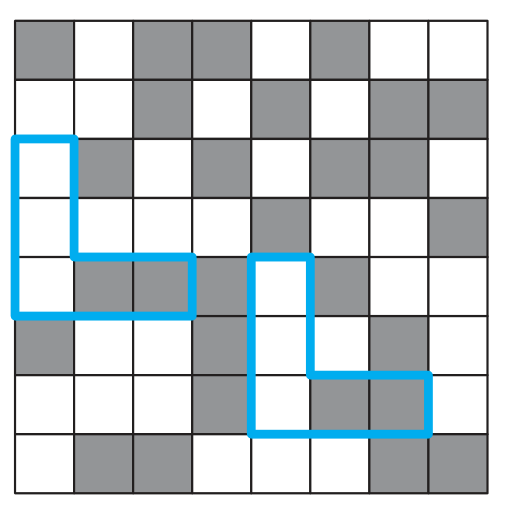
\includegraphics[scale=.5]{board.PNG}
\end{figure}
\vfill

\item Prove that $5^n-1$ is divisible by 4 for every positive integer $n$.
\vfill\null\pagebreak



\item What is wrong with the following proof?

\begin{thm}
	For every nonnegative integer $n$, $5n=0$.
\end{thm}

\begin{proof}
	We proceed by strong induction on $n$.
	For the base case, $n=0$, we have
	\begin{equation}
		5n = 5\cdot 0 = 0.
	\end{equation}
	For the inductive step, let $k$ be a nonnegative integer and suppose that $5n=0$ for all $n$ in the range $0\leq n\leq k$. Write $k+1 = i+j$ where $i$ and $j$ are integers satisfying $0\leq i,j\leq k$. We then apply the induction hypothesis to $i$ and $j$:
	\begin{equation}
		5(k+1) = 5(i+j) = 5i+5j = 0+0 = 0.
	\end{equation}
	By induction, $5n=0$ for all nonnegative integers $n$.
\end{proof}
\vfill

\item Recall that the Fibonacci numbers are defined by $F_1 = F_2 = 1$ and $F_{n+1} = F_n + F_{n-1}$ for all $n\geq 1$.

Prove that $F_1 + F_3 + F_5 + \cdots + F_{2n-1} = F_{2n}$ for all $n\geq 1$.
\vfill

\end{enumerate}

\end{document}